\chapter{Three Traits, Constructive Conflict, and the Growth of Trust}

This interview is short, but its structure is exact. We begin with a hiring question, move at once to a three-part filter, and then encounter a difficulty that the speaker does not hide: even the right people may argue intensely. The point of the chapter is to keep that order intact. First we identify the traits. Then we ask why those traits do not produce effortless harmony. Finally we see how, under the right conditions, disagreement becomes part of the mechanism by which a team discovers the best path forward and earns the confidence needed for independent judgment.

\section{The Hiring Question}

The opening question asks for the three most important traits to look for when assembling a leadership team or employing people for a company. That opening matters because it gives us a sharply bounded problem. We are not yet speaking about mission, charisma, or the mythology of founders. We are looking for a selection rule.

To keep the structure visible on the page, let us introduce a compact editorial shorthand:
\begin{equation}
T=\{H,I,C\},
\end{equation}
where \(H\) stands for honesty, \(I\) for intelligence, and \(C\) for coachability, that is, the ability to take constructive feedback.

This notation is only a way of keeping the lecture's first move orderly. The interview itself gives no weights and no scoring procedure. The natural reading is conjunctive: the three traits belong together.

\section{The Three-Trait Filter}

The speaker answers in a clipped sequence. We are told to work with honest people. Then with intelligent people. Then with people who can take constructive feedback. The movement is quick, but the third term immediately receives extra emphasis, and that is where the lecture begins to deepen.

A useful way to state the filter is
\begin{equation}
\mathcal{F}(p)=H(p)\wedge I(p)\wedge C(p),
\end{equation}
where \(\mathcal{F}(p)\) means that person \(p\) passes the basic team-building test. This is not a formula spoken in the interview; it is a disciplined reconstruction of the speaker's triad.

The third term is then restated in plainer language. One has to be coachable. And the correction comes at once: this does not apply only to the other person. It includes oneself. In that sense the third condition has a reflexive form:
\begin{equation}
C = C_{\text{self}} \wedge C_{\text{other}}.
\end{equation}

We should linger over this for a moment. Honesty and intelligence tell us something about the quality of a person taken individually. Coachability tells us something about what happens when that person is placed inside an actual working relationship. It is the first term in the lecture that points beyond selection and toward process.

\begin{itemize}
\item \(H\): we need people whose words, motives, and commitments can be relied upon.
\item \(I\): we need people who can understand the problem and reason about consequences.
\item \(C\): we need people who can receive correction without the work collapsing into defensiveness.
\end{itemize}

\section{The First Obstacle}

At this point the lecture could have remained a simple list. Instead it turns. The speaker says, in effect, that even with these traits in place, you are not always going to get along. That sentence is the hinge of the whole clip, because it prevents the first half from becoming a moral slogan.

\subsection{Question \& Answer}

\paragraph{Question.} If these are the right people to work with, why should there be so much friction among them?

\paragraph{Answer.} Because the absence of conflict is not the same thing as the presence of a strong team. Honest, intelligent, coachable people are often exactly the people who can argue hard about the path forward without treating the argument itself as proof that the relationship has failed.

That is why the lecture now leaves the list and turns to an early founding story. We are not changing subjects. We are asking what those three traits look like once real decisions begin pressing on the team.

\section{Argument as a Search Procedure}

The anecdote is introduced through a contrast between outside appearance and inside function. Others thought the founders were on the verge of destroying each other. The speaker's point is that the appearance was misleading. What they were doing was not merely clashing personalities; they were trying to flesh out the best path forward, or the best idea forward.

We can give this a careful name.

\begin{definition}
A disagreement is \emph{constructive} when its operative aim is clarification of the best path forward rather than personal victory.
\end{definition}

In that language, the lecture's central mechanism can be written schematically as
\begin{equation}
\text{constructive conflict}
\;\Rightarrow\;
\text{clearer best path}
\;\Rightarrow\;
\text{greater trust}
\;\Rightarrow\;
\text{more independent decisions}.
\end{equation}

This chain should be read with restraint. It is not a theorem of organizational science, and it is certainly not a universal law. It is a compact reconstruction of what the speaker is asserting in the interview. The point is that disagreement is reclassified. Once it is attached to the problem rather than to ego, it becomes a search procedure.

\begin{figure}[h]
\centering
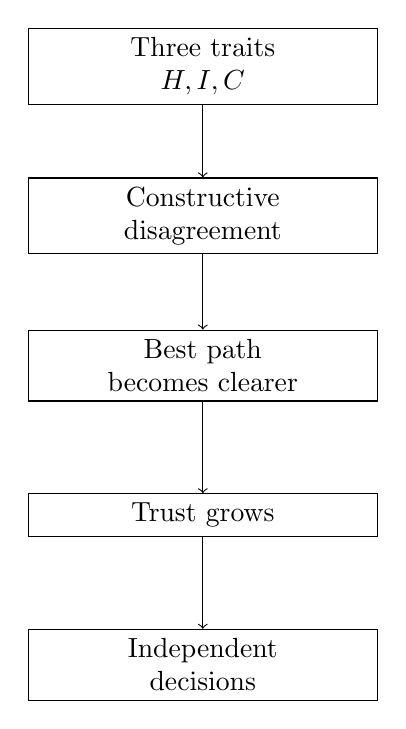
\begin{tikzpicture}
\node[draw, align=center, text width=4.2cm] (traits) at (0,0) {Three traits\\\(H,I,C\)};
\node[draw, align=center, text width=4.2cm] (conflict) at (0,-1.9) {Constructive\\disagreement};
\node[draw, align=center, text width=4.2cm] (path) at (0,-3.8) {Best path\\becomes clearer};
\node[draw, align=center, text width=4.2cm] (trust) at (0,-5.7) {Trust grows};
\node[draw, align=center, text width=4.2cm] (indep) at (0,-7.6) {Independent\\decisions};
\draw[->] (traits) -- (conflict);
\draw[->] (conflict) -- (path);
\draw[->] (path) -- (trust);
\draw[->] (trust) -- (indep);
\end{tikzpicture}
\caption{A narrow schematic reconstruction of the process described in the interview. The figure does not reproduce a board or slide; it simply makes the spoken logic explicit.}
\end{figure}

\section{The Packaging Example}

The lecture now narrows from the general mechanism to one specific case. In the early days of the company, the founders had strong arguments over which shade of red to use on the first product packaging. The detail is memorable because it is so small. The dispute was not over a merger, a financing, or an existential pivot. It was over packaging color.

That smallness is exactly why the example is useful. The speaker says that the issue itself turned out to be inconsequential. But the process of arguing through it was not inconsequential at all. The value of the episode lay not in the object being debated, but in what the debate revealed and trained.

So we should not read the story as a digression. We should read it as evidence for the mechanism already stated. A team does not build trust only in dramatic crises. It also builds trust in ordinary decisions, where irritation, repetition, and vanity can easily distort judgment. If the team can reason well there, then the conflict has informational value even when the underlying decision is small.

\section{Trust and Independent Judgment}

The clip closes by moving from mechanism to payoff. Through that process the founders became closer friends, trusted each other more, and came to make independent decisions with greater confidence in one another. In other words, constructive conflict changes the state of the relationship.

To write that idea in a compact mathematical form, let \(\tau_n\) denote the level of mutual trust after the \(n\)-th serious disagreement. Then the speaker's claim can be summarized schematically by the update rule
\begin{align}
\tau_{n+1} &= \tau_n + \Delta_n,\\
\Delta_n &>0 \qquad \text{when the disagreement stays oriented toward the best path forward.}
\end{align}

Again, the notation is editorial. The interview provides no measurement of trust, and the symbol \(\tau_n\) is introduced only to make the logic clearer. But the direction is faithful to the speaker's narration: the right kind of repeated argument adds to trust rather than subtracting from it.

We can unfold the logic step by step.
\begin{enumerate}
\item Select teammates for honesty, intelligence, and coachability.
\item Let real decisions be argued through rather than artificially smoothed over.
\item Keep the argument tied to the problem itself, so that criticism remains informative.
\item When this succeeds, each serious episode contributes a positive increment \(\Delta_n\) to the stock of mutual trust.
\item As trust increases, so does the ability to let one another make independent decisions without constant re-litigation.
\end{enumerate}

The final line of the interview gives the interpretation of the whole process. They needed to go through that early friction in order to reach that level of confidence with each other. This is an important closing qualification. The lecture is not praising conflict in itself. It is saying that some early conflict is the price of building a partnership that can later act with autonomy and confidence.

\section{Summary}

The lecture unfolds in a clean sequence. First comes the hiring question. Then comes the three-trait filter: honesty, intelligence, and coachability, with the explicit reminder that coachability includes oneself. Then comes the obstacle: the right people do not automatically produce easy harmony. The answer is that disagreement, when directed toward the best path forward, is not a breakdown of the team but one of the ways the team becomes strong. Even an argument over something as small as a shade of red can contribute to that process. Over time, repeated constructive conflict builds trust, and trust opens the door to independent judgment. That is the compact lesson of the clip: not simply whom to hire, but what kind of disciplined friction lets a good team become a durable one.